\documentclass[11pt, a4paper, USenglish]{article} % change ``USenglish'' to ``norsk'' if applicable.

\usepackage{kyblab} % Contains all included packages. See kyblab.sty.
\addbibresource{bibliography.bib} % Makes the bibliography file available to biblatex.

\begin{document}

% Titlepage
\title{\textbf{Helicopter lab report}\\ \textbf{TTK 4115}}
\author{Group 53\\Anders Granberg Drønnen 768686\\Bendik Steinkjer Standal 757944\\Filip Gornitzka Abelson 768687}
\date{October 2017}
\begin{titlepage}
    \maketitle
    \begin{figure}
    \centering
    \includegraphics[width=0.5\textwidth]{figures/itk_ntnu}\\
    Department of Engineering Cybernetics
    \end{figure}
    \thispagestyle{empty}
\end{titlepage}

% Abstract
\newpage
\begin{abstract} 
%\addcontentsline{toc}{section}{Abstract} % add this if you want the abstract in the table of contents.
  This document outlines a few important aspects of a lab report. It contains some advice on both content and layout. The \LaTeX{} source for this document is also published, and you can use it as a template of sorts for your own report. You can find an up to date version of the source at \url{https://github.com/ntnu-itk/labreport}. The main file, ``labreport.tex'', defines the structure of the document. The ``preamble.tex'' file is the document preamble, and contains a lot of informative comments. The document is based on work done by Tor Aksel Heirung for TTK4135, and is now under continuous improvement by Andreas L. Fl{\aa}ten and Kristoffer Gryte (happily accepting suggestions and contributions from the community).

When you write your own report, this section (the abstract) should contain a \emph{very} short summary of what the lab is about and what you have done.
\end{abstract}

\thispagestyle{empty} % Avoid page numbering on the abstract page.

% TOC
\newpage
\tableofcontents
\thispagestyle{empty} % Avoid page numbering on the table of contents.

% Main content
\newpage
\setcounter{page}{1}
\section{Introduction}\label{sec:intro}
Your introduction should contain an overview of the work you were assigned, as well as a few sentences putting the work into a larger perspective. You should also give a quick description of how the report is organized (as is done below).

You should of course put most of the work into doing good work in the lab and then presenting it in the report. When presenting your work in the report, both content and presentation/layout matters. Since your only way of communicating your good effort in the lab is through writing about it here, the way you write about it is essential. This means that even if you have the very best controller but describe it poorly, you will probably not be rewarded for the good results. A plot showing perfect control is worth very little if it is not accompanied by a clear description of what it represents.

Layout is naturally less important than content, but it still matters. You can think of report writing like selling an apartment; when you present your apartment for potential buyers you will of course clean the apartment and make it good looking. How clean the apartment is does of course not determine its value, but it is still important since it influences the subjective value your buyers will put on the apartment. 

\subsection{Software}
You are of course free to use whatever software you want for report writing. You can also submit a handwritten report, although this is probably not a great idea if your handwriting can be hard to read. 

You can also use Word or a similar word processor. However, it is next to impossible to achieve decent layout with Word. The support for vector graphics (discussed later) is extremely poor, and text tends to look pretty bad (bad support for kerning and ligatures). Furthermore, math is both time consuming and difficult to input, and tends to look very ugly. In general, a report written in Word looks like a draft.

It is strongly recommended to use Latex. Unless you tweak the layout too much, your report will almost certainly look very good. Although it can take a bit of effort to get started, it is also much quicker to use than Word and similar programs. The support for math and vector graphics is also great.

If you are new to Latex, you can have a look at the source for this document to get started. You can also look at the presentation by~\cite{Berland2010} (in Norwegian) or consult~\cite{Oetiker2011}. Another good reason to learn Latex is that you probably don't want to write your master's thesis in something like Word, doing so would likely be very frustrating. Being reasonably fluent in Latex before you get that far will make your thesis work much smoother.

Some of you are probably fluent in Latex and might plan to write the report using it. Please resist the temptation (if any) to change the fonts, make super fancy headers (they are not necessary for a report like this), change the margins, change the paragraph indentation and/or spacing, and similar things.

A great tool for collaborating on Latex documents is ShareLaTeX at \url{https://www.sharelatex.com/}; if you use this you won't have to install anything on your computer. Texmaker at \url{http://www.xm1math.net/texmaker/} is a good cross-platform editor. Some people like Lyx, which is a Latex editor that behaves a little bit like Word. If you prefer to compile your Latex document on the command line, the latexmk \url{https://www.ctan.org/pkg/latexmk} command is a great tool included in most TeX distributions. There is also a simple Vim plugin that uses latexmk as its backend called LaTeX-BoX \url{https://github.com/LaTeX-Box-Team/LaTeX-Box}.

\subsection{Other Comments}
Unless you have a very good reason not to, you should write the report in English. If you have problems with Latex, the solution is usually just a few Google searches away.

This report is organized as follows: \Cref{sec:prob_descr} contains some course specific equations, and some tips on how to create illustrations. Several \LaTeX{} tips can be found in \Cref{sec:latex_tips}, such as how to create a table and matrix equations. \Cref{sec:figures} contains some advice on using plots from MATLAB\@. The closing remarks are in~\Cref{sec:conclusion}, respectively. \Cref{sec:matlab} contains a MATLAB file while \Cref{sec:simulink} shows an example Simulink diagram. The Bibliography can be found at the end, on page~\pageref{sec:bibliography}.

\section{Part I - Mathematical modeling}\label{sec:part1}

\subsection{Problem 1}
\begin{subequations} \label{eq:motor}
    \begin{gather}
        F_f = K_f V_f \label{eq:motor_front} \\
        F_b = K_f V_b \label{eq:motor_back}
    \end{gather}
\end{subequations}
\begin{subequations} \label{eq:model}
    \begin{gather}
        J_p \ddot{p} = L_1 V_d \label{eq:model_pitch}\\
        J_e \ddot{e} = L_2 \cos(e) + L_3 V_s \cos(p) \label{eq:model_elev}\\
        J_{\lambda} \ddot{\lambda} = L_4 V_s \cos(e) \sin(p) \label{eq:model_travel}
    \end{gather}
\end{subequations}
By using Newton's second low for rotation, we can compute the equations of motion, in the form as stated above. We will insert equation \eqref{eq:motor_front} and \eqref{eq:motor_back}.
\begin{equation} \label{eq:newton2rot}
    J \alpha = \sum{\tau}
\end{equation}
We will begin with the equation for pitch. The torques generated by gravity cancel each other out, so we end up with the torques generated by the motors.
\begin{gather*}
    J_p \ddot{p} = l_p F_{g,b} - l_p F_{g,f} + l_p F_f - l_p F_b \\
    = l_p K_f V_f - l_p K_f V_b = l_p K_f (V_f - V_b) \\
    \implies J_p \ddot{p} = L_1 V_d
\end{gather*}
Now we will look at the equation for elevation. We must use basic trigonometry to find the right components of the forces. As we can see, the forces are dependant on both pitch angle and elevation angle.
\begin{gather*}
    J_p \ddot{e} = l_c F_{g,c} \cos(e) + l_h (F_f \cos(p) + F_b \cos(p) - l_h F_{g,f} \cos(e) - l_h F_{g,b} \cos(e) \\
    = l_c F_{g,f} \cos(e) + l_h K_f \cos(p) (V_f + V_b) - 2 l_h m_p g \cos(e) \\
    = g(l_c m_c - 2 l_h m_p) \cos(e) + l_h K_f V_s \cos(p) \\
    \implies J_e \ddot{e} = L_2 \cos(e) + L_3 V_s \cos(p)
\end{gather*}
The last equation is the one for travel. Once again, we must use basic trigonometry to find the force and lever arm which are orthogonal. 
\begin{gather*}
    J_\lambda \ddot{\lambda} = \tau_f - \tau_b \\
    = - l_h \cos(e) F_f \sin(p) - l_h \cos(e) F_b \sin(p)\\
    = - l_h K_f (V_f + V_b) \cos(e) \sin(p) = - l_h K_f V_s \cos(e) \sin(p)\\
    \implies J_\lambda \ddot{\lambda} = L_4 V_s \cos(e) \sin(p)
\end{gather*}
Now we have expressions for the constants $L_{1-4}$:
\begin{subequations}\label{eq:constants-L}
    \begin{align}
        & L_1 = l_p K_f \label{eq:constant-L1}\\
        & L_2 = g (l_c m_c - 2 l_h m_p) \label{eq:constant-L2}\\
        & L_3 = l_h K_f \label{eq:constant-L3} \\
        & L_4 = - L_3 = - l_h K_f \label{eq:constant-L4}
    \end{align}
\end{subequations}
\begin{subequations}\label{eq:motor_voltage}
    \begin{gather}
        V_s = V_f + V_b \label{motor_voltage_sum}\\
        V_d = V_f - V_b \label{motor_voltage_difference}
    \end{gather}
\end{subequations}
\subsection{Problem 2}\label{subsec:P1p2}
To be able to control our helicopter, we must linearize the equation of motion. We will linearize the model around the point $(p,e,\lambda)^T=(p^*,e^*,\lambda^*)^T$ with $p^*=e^*=\lambda^*=0$. Now we determine the voltages $V_s^*$ and $V_d^*$, such that for all time $\dot{p} = \dot{e} = \dot{\lambda} = 0$. 
This implies that $\ddot{p} = \ddot{e} = \ddot{\lambda} = 0$ for all time. \\
\\Equation \eqref{eq:model_pitch} yields;
\begin{align}
    J_p \cdot 0 = L_1 V_d \implies V_d^* = 0
\end{align}
Equation \eqref{eq:model_elev} yields;
\begin{align}
    J_e \cdot 0 &= L_2 \cos(0) + L_3 V_s^* \cos(0) \nonumber \\
    L_3 V_s^* &= - L_2 \implies V_s^* = -\frac{L_2}{L_3}\label{eq:vs_tilde}
\end{align}
We use the following coordinate transformation to linearize and rewrite the equations of motion. 
\begin{equation}\label{eq: coord_trans}
    \begin{bmatrix} 
        \tilde{p} \\ \tilde{e} \\ \tilde{\lambda}
    \end{bmatrix}
    =
    \begin{bmatrix} 
        p \\ e \\ \lambda
    \end{bmatrix}
    -
    \begin{bmatrix} 
        p^* \\ e^* \\ \lambda^*
    \end{bmatrix}
    \text{ and }
    \begin{bmatrix}
        \tilde{V_s} \\ \tilde{V_d}
    \end{bmatrix}
    =
    \begin{bmatrix}
        V_s \\ V_d
    \end{bmatrix}
    -
    \begin{bmatrix}
        V_s^* \\ V_d^*
    \end{bmatrix}
\end{equation}



\textbf{DE UNDER BØR KANSKJE SETTES ET ANNET STED??}
\begin{subequations} \label{eq:moments_inertia}
    \begin{align}
        & J_p = 2 m_p l_p^2 \\
        & J_e = m_c l_c^2 + 2 m_p l_h^2 \\
        & J_\lambda = m_c l_c^2 + 2 m_p (l_h^2 + l_p^2)
    \end{align}
\end{subequations}
\begin{subequations}
    \begin{align}
        & \ddot{\tilde{p}} = \frac{L_1}{J_p} \tilde{V_d} \label{eq:trans_model_pitch}\\
        & \ddot{\tilde{e}} = \frac{L_2}{J_e} \cos(\tilde{e}) + \frac{L_3}{J_e}(\tilde{V_s} - \frac{L_2}{L_3}) \cos(\tilde{p})\label{eq:trans_model_elev} \\
        & \ddot{\tilde{\lambda}} = \frac{L_4}{J_\lambda } (\tilde{V_s}-\frac{L_2}{L_3}) \cos(\tilde{e}) \sin(\tilde{p})\label{eq:trans_model_travel}
    \end{align}
\end{subequations}
We set up a state-space model on the following form and linearize the model around $\mathbf{x}_0 = \mathbf{0}$ and $\mathbf{u}_0 = (0, -\frac{L_2}{L_3})^T$.
\begin{equation*}
    \mathbf{\dot{x}} = \mathbf{Ax} + \mathbf{Bu}
\end{equation*}
Where, 
\begin{equation*}
    \mathbf{x} = 
    \begin{bmatrix}
        x_1 \\ x_2 \\ \vdots \\ x_6
    \end{bmatrix}
    =
    \begin{bmatrix}
        \tilde{p} \\ \dot{\tilde{p}} \\ \tilde{e} \\ \dot{\tilde{e}} \\ \tilde{\lambda} \\ \dot{\tilde{\lambda}} \\ 
    \end{bmatrix}
    \text{ and }
    \mathbf{u} =
    \begin{bmatrix}
        \tilde{u_1} \\ \tilde{u_2}
    \end{bmatrix}
    =
    \begin{bmatrix}
        \tilde{V_s} \\ \tilde{V_d}
    \end{bmatrix}
\end{equation*}
Using equation \eqref{eq:trans_model_pitch}, \eqref{eq:trans_model_elev} and \eqref{eq:trans_model_travel} we get the following expression for $\mathbf{\dot{x}}$.
\begin{equation*}
    \mathbf{\dot{x}} = 
    \begin{bmatrix}
        f_1 \\ f_2 \\ \vdots \\ f_6
    \end{bmatrix}
    =
    \begin{bmatrix}
        x_2 \\ \frac{L_1}{J_p}u_2 \\ \frac{L_2}{J_e}\cos(x_3) + \frac{L_3}{J_e} u_1 \cos(x_1) \\ x_6 \\ \frac{L_4}{J_\lambda}u_1 \cos(x_3) \sin(x_1)
    \end{bmatrix}
\end{equation*}
Now we can find the matrices \textbf{A} and \textbf{B}.
\begin{gather*}
    \mathbf{A} = \frac{\partial \mathbf{f}}{\partial \mathbf{x}} = 
    \left.
    \begin{bmatrix}
        \frac{\partial f_1}{\partial x_1} & \cdots &\frac{\partial f_1}{\partial x_6} \\
        \vdots & \ddots & \vdots \\
        \frac{\partial f_6}{\partial x_1} & \cdots & \frac{\partial f_6}{\partial x_6}
    \end{bmatrix}
    \right|_{\mathbf{x_0}, \mathbf{u_0}}
    \text{, }
    \mathbf{B} = \frac{\partial \mathbf{f}}{\partial \mathbf{u}} = 
    \left.
    \begin{bmatrix}
        \frac{\partial f_1}{\partial u_1} & \frac{\partial f_1}{\partial u_2} \\
        \frac{\partial f_6}{\partial u_1} & \frac{\partial f_6}{\partial u_2}
    \end{bmatrix}
    \right|_{\mathbf{x_0}, \mathbf{u_0}}
\end{gather*}
Calculating the partial derivatives and inserting for the points we are linearizing about, we get
\begin{gather}
    \mathbf{A} = 
    \begin{bmatrix}
        0 & 1 & 0 & 0 & 0 & 0 \\
        0 & 0 & 0 & 0 & 0 & 0 \\
        0 & 0 & 0 & 1 & 0 & 0 \\
        0 & 0 & 0 & 0 & 0 & 0 \\
        0 & 0 & 0 & 0 & 0 & 1 \\
        -\frac{L_2 L_4}{J_\lambda L_3} & 0 & 0 & 0 & 0 & 0 \\
    \end{bmatrix}
    \text{ and }
    \mathbf{B} =
    \begin{bmatrix}
        0 & 0 \\
        0 & \frac{L_1}{J_p} \\
        0 & 0 \\
        \frac{L_3}{J_e} & 0\\
        0 & 0 \\
        0 & 0 \\
    \end{bmatrix}
\end{gather}
And this gives us the linearized equations:
\begin{subequations} \label{eq:lin_model}
    \begin{align}
        &\tilde{\ddot{p}} = K_1 \tilde{V_d} \label{eq:lin_model_pitch}\\
        &\tilde{\ddot{e}} = K_2 \tilde{V_s} \label{eq:lin_model_elev}\\
        &\tilde{\ddot{\lambda}} = K_3 \tilde{p} \label{eq:lin_model_travel}
    \end{align}
\end{subequations}
where
\begin{gather}
    K_1 = \frac{L_1}{J_p}, K_2 = \frac{L_3}{J_e} \text{ and } K_3 = -\frac{L_2 L_4}{L_3 J_\lambda}
\end{gather}

\subsection{Problem 3}
?????

\subsection{Problem 4}
Now we want to determine the motor voltage constant, $K_f$, by measuring the value of $V_s = V_s^*$ which makes the helicopter maintain the equilibrium value $e = e^* = 0$. We measured the voltage to be $V_s = V_s^* = 6.75 \text{ V}$. 
\\From equation \eqref{eq:vs_tilde}, we have that $V_s^* = -\frac{L_2}{L_3}$. Furthermore, we can expand this expression using equation \eqref{eq:constant-L2} and equation \eqref{eq:constant-L3}, then solve for $K_f$ and finally insert the constant values and the measured value for $V_s^*$. 
\begin{gather}
    V_s^* = -\frac{L_2}{L_3} = \frac{g(2 l_h m_p - l_c m_c)}{l_h K_f}\nonumber\\
    \implies K_f = \frac{g(2 l_h m_p - l_c m_c)}{l_h V_s^*} = 0.148
\end{gather}
\section{Part II - Monovariable control}
\subsection{Problem 1 - Pitch angle PD controller}
A PD controller is to be added to control the pitch angle $p$. This controller is given as:
\begin{gather}
    \tilde{V}_d = K_{pp}(\tilde{p}_c-\tilde{p})-K_{pd}{\dot{\tilde{p}}}\label{eq:pd-controller}
\end{gather}
From equation \eqref{eq:lin_model_pitch} we see that $\tilde{V}_d = \frac{\ddot{\tilde{p}}}{K_1}.$ Substituting this into the equation \eqref{eq:pd-controller} for the PD controller gives:
\begin{gather*}
    \tilde{\ddot{p}} = K_1(K_{pp}(\tilde{p}_c - \tilde{p}) - K_{pd}\tilde{\dot{p}} \\
    \ddot{\tilde{p}} + K_1K_{pd}\dot{\tilde{p}} + K_1K_{pp}\tilde{p} = K_1 K_{pp} \tilde{p}_c
\end{gather*}
Using the Laplace transform and assuming $\tilde{p}(0) = \dot{\tilde{p}}(0) = 0$, gives us the transfer function:
\begin{gather*}
    s^2\tilde{p}(s) + sK_1K_{pd}\tilde{p}(s) + K_1K_{pp}\tilde{p}(s) = K_1K_{pp}\tilde{p}_c(s) \\
    \tilde{p}(s)(s^2 + sK_1K_{pd} + K_1K_{pp}) = K_1K_{pp}\tilde{p}_c(s) \\
    \frac{\tilde{p}(s)}{\tilde{p}_c(s)} = \frac{K_1K_{pp}}{s^2 + K_1K_{pd}s + K_1K_{pp}}
\end{gather*}
The linearized pitch dynamics can be regarded as a second-order linear system, generally given by the transfer function:
\begin{gather*}
    \frac{K\omega_0^2}{s^2 + 2\zeta\omega_0s + \omega_0^2}
\end{gather*}
We wish to obtain critical damping, in order to get the system to return to its equilibrium in the minimum amount of time without overshooting. Hence, we set $\zeta = 1$. The general transfer function for this type of system is given by:
\begin{gather*}
    \frac{K\omega_0^2}{s^2 + 2\omega_0s + \omega_0^2}
\end{gather*}
Comparing the transfer function of our system (equation number) to the general one (equation number), gives the following equations for the regulator parameters:
\begin{gather*}
    K_{pp} = \frac{\omega_0^2}{K_1} \text{ and } K_{pd} = 2 \frac{\omega_0}{K_1}
\end{gather*}
Now, we need to tune the controller gains $K_{pp}$ and $K_{pd}$. Our goal is to make the controller regulate the pitch angle rapidly to its desired value, without excessive oscillations. The natural frequency $\omega_o$ decides the rapidness of the pitch regulation. Increasing $\omega_o$ will make the controller react to pitch changes faster. This is because we move the poles of the system further into the left plane, seen by examining the the denominator of (equation number):
\begin{gather*}
    (s + \omega_0)^2
\end{gather*}
 Looking at the expressions for  $K_{pp}$ and $K_{pd}$ (equation number) and (equation number), we see that they're both dependant of $\omega_0$. Unsurprisingly, this means that tuning of the controller gains influences the closed-loop eigenvalues and the pitch response. A higher value for $K_{pp}$ for instance, will move the eigenvalues to the left in the complex plane, and give faster pitch response. However, there is a limit to how much the controller gains, and thus the natural frequency, may be increased. Increasing it too much may damage the helicopter, or make it unstable. 
 Through a process starting with initial guesstimates, followed by tuning by trial and error, we found values that gave us a satisfying response:
\begin{gather*}
    K_{pp} = 14 \\ 
    K_{pd} = 9.765
\end{gather*}

EVENTUELT DISKUSJON OM PD VS. FEED FORWARD.

\subsection{Problem 2 - Travel rate P controller}
We now aim to control the travel rate $\dot{\tilde{\lambda}}$ using a simple P controller:
\begin{gather*}
    \tilde{p}_c = K_{rp}(\dot{\tilde{\lambda}}_c - \dot{\tilde{\lambda}})
\end{gather*}
where $K_{rp} < 0$. We now assume that the pitch angle is controlled perfectly, that is $\tilde{p} = \tilde{p}_c$. Substituting (equation number) into the equation for the P controller gives:
\begin{gather*}
    \ddot{\tilde{\lambda}} = K_3(K_{rp}(\dot{\tilde{\lambda}}_c - \dot{\tilde{\lambda}})) \\ 
    \ddot{\tilde{\lambda}} + K_3K_{rp}\dot{\tilde{\lambda}} = K_3K_{rp}\dot{\tilde{\lambda}}_c
\end{gather*}
Using the Laplace transform and assuming  $\tilde{\lambda}(0) = \dot{\tilde{\lambda}}(0) = 0$, gives us the transfer function from the reference $\dot{\tilde{\lambda}}_c$ to the travel rate $\dot{\tilde{\lambda}}$:
\begin{gather*}
    s\dot{\tilde{\lambda}}(s) + K_3K_{rp}\dot{\tilde{\lambda}}(s) = K_3K_{rp}\dot{\tilde{\lambda}}_c(s) \\
    \dot{\tilde{\lambda}}(s)(s + K_3K_{rp}) = K_3K_{rp}\dot{\tilde{\lambda}}_c(s) \\
    \frac{\dot{\tilde{\lambda}}(s)}{\dot{\tilde{\lambda}}_c(s)} = \frac{K_3K_{rp}}{s + K_3K_{rp}}
\end{gather*}
The transfer function can be written as:
\begin{gather*}
    \frac{ \dot{\tilde{\lambda}}(s)}{\dot{\tilde{\lambda}}_c(s)} = \frac{\rho}{s + \rho}
\end{gather*}
where $\rho = K_3K_{rp}$. We tested the helicopter's response for different values for $K_{rp}$, and found that $K_{rp} = -1.2$ gave a fast and accurate response.  
\section{Part III - Multivariable control}\label{sec:part3}
\subsection{Problem 1 - State-Space Representation}
We put the system in a state-space formulation on the form:
\begin{gather*}
    \mathbf{\dot{x}} = \mathbf{Ax} + \mathbf{Bu}
\end{gather*}
where A and B are matrices, and our state and input vector are: 
\begin{gather*}
    \mathbf{x} = 
    \begin{bmatrix}
        \tilde{p}\\\tilde{\dot{p}}\\\tilde{\dot{e}}
        \end{bmatrix}
     \text{  and  } \mathbf{u} = 
    \begin{bmatrix} \tilde{V_s}\\\tilde{V_d} \end{bmatrix}
\end{gather*}
This gives us the following state-space model:
\begin{gather*}
     \begin{bmatrix}
        \tilde{\dot{p}}\\\tilde{\ddot{p}}\\\tilde{\ddot{e}}
    \end{bmatrix}
    \text{ + } \begin{bmatrix}
        0 & 1 & 0 \\
        0 & 0 & 0 \\
        0 & 0 & 0 \\ \end{bmatrix}
    \begin{bmatrix}
        \tilde{p}\\\tilde{\dot{p}}\\\tilde{\dot{e}}
    \end{bmatrix}
    \text{ = } \begin{bmatrix}
        0 & 0 \\
        0 & K_1 \\
        K_2 & 0 \\
    \end{bmatrix}
    \begin{bmatrix} \tilde{V_s}\\\tilde{V_d} \end{bmatrix}
\end{gather*}

\subsection{Problem 2 - Linear Quadratic Regulator}
We now aim to track the reference $\mathbf{r}
= \begin{bmatrix} \tilde{p_c,} & \tilde{\dot{e_c}}
\end{bmatrix}^T$ for the pitch angle $\tilde{p}$ and elevation rate $\dot{\tilde{e}}$. The reference values $\tilde{p}_c$ and $\dot{\tilde{e}}_c$ are given by the joystick, the x-axis and y-axis respectively. Firstly, we examine if the system is controllable. The controllability matrix is given by:
\begin{gather*}
    \mathcal{C} = 
    \begin{bmatrix} \mathbf{B} & \mathbf{AB} &
    \mathbf{A^2B} \end{bmatrix}
    = \begin{bmatrix}
    0 & 0 & 0 & K_1 & 0 & 0 \\
    0 & K_1 & 0 & 0 & 0 & 0 \\
    K_2 & 0 & 0 & 0 & 0 & 0
    \end{bmatrix}
\end{gather*}
We see that $\mathcal{C}$ has full rank, which means that the system is controllable. In order to actually control the system, we implement a controller of the form:
\begin{gather*}
    \mathbf{u} = \mathbf{Pr} - \mathbf{Kx}
\end{gather*}
In the controller, $\mathbf{r}$ is the reference given by the joystick output. The matrix $\mathbf{K}$ corresponds to the linear quadraric regulator (LQR) for which the control input $\mathbf{u} = -\mathbf{Kx}$ optimizes the cost function
\begin{gather*}
    \mathit{J} = \int_{0}^{\infty}(\mathbf{x}^T(t)
    \mathbf{Qx}(t) + \mathbf{u}^T(t)\mathbf{Ru}(t))
    \mathit{dt}
\end{gather*}
The matrix $\mathbf{K}$ is obtained by using the MATLAB command K = lqr(A,B,Q,R), where $\mathbf{Q}$ and $\mathbf{R}$ are weighting matrices. For simplicity, $\mathbf{Q}$ and $\mathbf{R}$ are diagonal. When deciding their elements we started with an initial guess, and tuned from there. We looked for values making the helicopter fast and accurate, and ended up with the following:
\begin{gather*}
    \mathbf{Q} = \begin{bmatrix}
    91.2 & 0 & 0 \\ 
    0 & 50 & 0 \\
    0 & 0 & 100 \end{bmatrix}\textbf{, } \mathbf{R} = \begin{bmatrix} 1 & 0 \\ 0 & 1 \end{bmatrix}
\end{gather*}
Our state-space model with the controller is
\begin{gather*}
     \mathbf{\dot{x}} = \mathbf{Ax} + \mathbf{B}(\mathbf{Pr} - \mathbf{Kx})
\end{gather*}
We want to obtain a solution such that  \( \mathbf{y}(t) \rightarrow \mathbf{r} \)  as t \(\rightarrow \infty\). When the output gets stable,  
\(\mathbf{\dot{x}} \rightarrow 0\). We get:
\begin{gather*}
    0 = \mathbf{Ax_\infty} + \mathbf{B}(\mathbf{Pr} - \mathbf{Kx_\infty)} \\
    (\mathbf{A} - \mathbf{BK})\mathbf{x_\infty} = -\mathbf{BPr} \\
    \mathbf{x_\infty} = (\mathbf{BK} - \mathbf{A})^{-1}
    \mathbf{BPr}
\end{gather*}
Substituting this into \(\mathbf{y_\infty} = \mathbf{Cx_\infty}\) yields:      
\begin{gather*}
    \mathbf{y_\infty} = 
    \begin{bmatrix} \mathbf{C}(\mathbf{BK} - \mathbf{A})^{-1} \mathbf{B}\end{bmatrix}\mathbf{Pr}
\end{gather*}
which gives:
\begin{gather*}
    \mathbf{P} = 
    \begin{bmatrix}\mathbf{C}(\mathbf{BK} - \mathbf{A})^{-1}\mathbf{B}\end{bmatrix}^{-1}
\end{gather*}
Our \textbf{K} and \textbf{P}:
\begin{gather*}
    \mathbf{K} = \begin{bmatrix}
    0 & 0 & 10 \\
    9.5499 & 9.0841 & 0 \end{bmatrix}\textbf{, } \mathbf{P} =
    \begin{bmatrix} 0 & 10 \\ 9.5499 & 0 \end{bmatrix}
\end{gather*}

KOMMENTERE KONTROLLERVALG

\subsection{Problem 3 - PI controller}
We now modify the controller to include an integral effect for the elevation rate and the pitch angle. Including an integral effect makes our controller a PI controller, and results in two additional states. We call the new states $\gamma$ and $\zeta$, and their differential equations are given by:
\begin{gather*}
    \dot{\gamma} = \tilde{p} - \tilde{p_c}\\
    \dot{\zeta} = \dot{\tilde{e}} - \dot{\tilde{e_c}}
\end{gather*}
The state vector and the input vector are now given by:
\begin{gather*}
    \mathbf{x} = \begin{bmatrix}
    \tilde{p} \\ \tilde{\dot{p}} \\
    \dot{\tilde{e}} \\ \gamma \\ \zeta \end{bmatrix}
    \text{ and } \mathbf{u} = \begin{bmatrix}
    \tilde{V_s} \\ \tilde{V_d} \end{bmatrix}
\end{gather*}

HER MÅ VI HA PLOTS HVOR VI SAMMENLIGNER HELIKOPTERETS RESPONS MED OG UTEN INTEGRALEFFEKT. EVT. NYE Q,R OG K MED FORKLARING. 










\section{Part IV - State Estimation}\label{sec:part4}

\subsection{Problem 1 - State-space formulation}\label{subsec:P4p1}
We wish to derive a state-space formulation from the system of linearized equations derived in \ref{subsec:P1p2} on the form

\begin{equation}\label{eq:state-space}
\begin{split}
    \mathbf{\dot{x}} &= \mathbf{Ax + Bu}\\
    \mathbf{y} &= \mathbf{Cx}
\end{split}
\end{equation}
where \textbf{A, B} and \textbf{C} are matrices defined below. The state vector, the input vector and the output vector are now given by:

\begin{align}\label{eq:states_part4}
    \textbf{x} &= \begin{bmatrix} \tilde{p} \\ \dot{\tilde{p}} \\ \tilde{e} \\ \dot{\tilde{e}} \\ \tilde{\lambda} \\ \dot{\tilde{\lambda}} \end{bmatrix}, &\textbf{u} &= \begin{bmatrix} \tilde{V_{s}} \\ \tilde{V_{d}} \end{bmatrix}, &\mathbf{y} &= \begin{bmatrix} \tilde{p} \\ \tilde{e} \\ \tilde{\lambda} \end{bmatrix}
\end{align}
From the output equation and the state vector, we can directly see that the matrix \textbf{C} is given by 
\begin{equation}
    \mathbf{C} = 
    \begin{bmatrix}
    1 & 0 & 0 & 0 & 0 & 0 \\
    0 & 0 & 1 & 0 & 0 & 0 \\
    0 & 0 & 0 & 0 & 1 & 0
    \end{bmatrix}
\end{equation}
Furthermore, using the equations \eqref{eq:lin_model_pitch}-\eqref{eq:lin_model_travel}, the state equation can be written as
\begin{equation}\label{eq:state_matrices_P4p1}
    \mathbf{\dot{x}} = 
    \begin{bmatrix} 
        \dot{\tilde{p}} \\ 
        \ddot{\tilde{p}} \\ 
        \dot{\tilde{e}} \\ 
        \ddot{\tilde{e}} \\ 
        \dot{\tilde{\lambda}}\\ 
        \ddot{\tilde{\lambda}} 
    \end{bmatrix} = 
    \begin{bmatrix} 
        x_{2}\\ 
        K_1\tilde{V_d}\\ 
        x_4\\ 
        K_2\tilde{V_s}\\ 
        x_6\\ 
        K_3 x_1 
    \end{bmatrix} =
    \underbrace{
    \begin{bmatrix}
        0 & 1 & 0 & 0 & 0 & 0 \\
        0 & 0 & 0 & 0 & 0 & 0 \\
        0 & 0 & 0 & 1 & 0 & 0 \\
        0 & 0 & 0 & 0 & 0 & 0 \\
        0 & 0 & 0 & 0 & 0 & 1 \\
        K_3 & 0 & 0 & 0 & 0 & 0
    \end{bmatrix}}_\mathbf{A}\mathbf{x} + 
    \underbrace{
    \begin{bmatrix}
        0 & 0 \\
        0 & K_1 \\
        0 & 0 \\
        K_2 & 0 \\
        0 & 0 \\
        0 & 0 
    \end{bmatrix}}_\mathbf{B}\mathbf{u}
\end{equation}

\subsection{Problem 2 - Linear observer}\label{subsec:P4p2}
In order to examine the observability of the system, we calculate the observability matrix using
\begin{equation}\label{eq:obs_matrix}
    \mathcal{O} = 
    {\begin{bmatrix}\mathbf{C}\\ \mathbf{CA}\\ \mathbf{CA^2}\\ \vdots \\ \mathbf{CA^{n-1}}\end{bmatrix}}
\end{equation}
We have learned from \cite{Lecture_5} that the criteria for a system to be observable is that equation \eqref{eq:obs_matrix} has full rank. In our case, this is achieved after the two first computations in the observability matrix:
\begin{equation}\label{eq:obs_matrix_calc}
    {\mathcal {O}}_{2}=
    {\begin{bmatrix}
        1 & 0 & 0 & 0 & 0 & 0\\
        0 & 0 & 1 & 0 & 0 & 0\\
        0 & 0 & 0 & 0 & 1 & 0\\
        0 & 1 & 0 & 0 & 0 & 0\\
        0 & 0 & 0 & 1 & 0 & 0\\
        0 & 0 & 0 & 0 & 0 & 1
    \end{bmatrix}}
\end{equation}
Hence, our system is indeed observable.\\
\\
Next, we wish to create a linear observer for the system of the form:
\begin{equation}\label{observer_system}
    \mathbf{\dot{\hat{x}} = A\hat{x} + Bu + L(y - C\hat{x})}
\end{equation}
where \textbf{L} is the observer gain matrix.
Because the system is observable, we have the opportunity to place the poles of the system where we want in order to obtain an optimal response. We can do this by choosing an appropriate gain matrix \textbf{L}. The estimator $\mathbf{\hat{x}}$ has the same poles as $\mathbf{A - LC}$. Generally, we want the error dynamics to be faster than the system itself. In practice, this means that the poles of $\mathbf{A - LC}$ should be placed further into the left half plane than the poles of $\mathbf{A - BK}$, which represents the system dynamics. We place the estimator poles on a circular arc in the left half plane, shown in \cref{fig:Pole_placement_P4p2}. The radius of this arc is determined by a multiple of the distance to the most negative pole of the original system. MATLAB provides a simple function place() to compute the observer gain matrix \textbf{L}. MATLAB code for implementing this is shown in \cref{subsec:P4p2_init.m}.
\begin{figure}[htb]
	\centering
		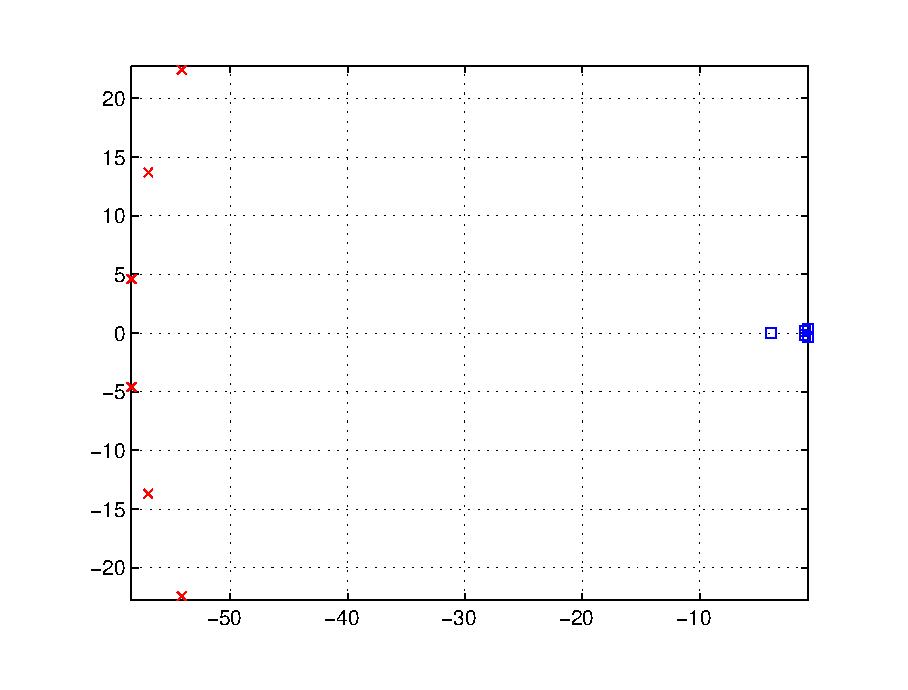
\includegraphics[width=0.8\textwidth]{figures/Pole_placement_P4p2_integral.eps}
	\caption{Pole placement for the system with integral controller from part III. The system poles are located in blue on the right, while the observer poles are seen in red.}
\label{fig:Pole_placement_P4p2}
\end{figure}
\\
Choosing a ideal gain matrix will be very important for this system, because although we want a fast estimator, the further into the left half plane the estimator poles are located, the more we will amplify noise in the measurements. In our project, we ended up placing the estimator poles on an arc with radius 13 times the distance of the most negative pole from the original system.\\
\\As in part 3, we tried tuning with different values for the matrices \textbf{Q} and \textbf{R} until the desired behaviour was reached. We seemed however to get the best results with similar values as in part III, see \cref{eq:P3_weighting_matrices}. With the computed gain matrix
\begin{equation}\label{eq:L_P4p2}
\mathbf{L} = \begin{bmatrix}
97,94 & 6,20 & -13,90\\
2476,40 & 318,65 & -725,98\\
-2,47 & 98,99 &	1,78\\
-114,14 & 2600,04 &	80,90\\
15,36 & 2,71 & 96,90\\
786,98 & -148,13 & 2412,86
\end{bmatrix}
\end{equation}
we were able to reach satisfying results with both controllers from part III. Plots of the estimated values versus the real values for both controllers are shown below, first for the regular P controller in \cref{fig:P4p2_states_vs_obs} and then the PI controller in \cref{fig:P4p2_int_states_vs_obs}. The Simulink-diagram to show the implementation of the observer is included in \cref{fig:P4_observer}, \cref{sec:simulink}
\subsection{Problem 3 - Observer without pitch}\label{subsec:P4p3}
We aim to control our system by only measuring $\tilde{e}$ and $\tilde{\lambda}$. The output \textbf{y} and output matrix \textbf{C} becomes:
\begin{equation}\label{eq:y_P4p3}
\mathbf{y} = 
\begin{bmatrix}
\tilde{e}\\
\tilde{\lambda}
\end{bmatrix}
\end{equation}
and
\begin{equation}\label{eq:C_P4p3}
\mathbf{C} = 
    \begin{bmatrix}
    0 & 0 & 1 & 0 & 0 & 0 \\
    0 & 0 & 0 & 0 & 1 & 0 
    \end{bmatrix}
\end{equation}
Again, as in \ref{subsec:P4p2}, we use equation \eqref{eq:obs_matrix} to examine if the system is observable:
\begin{equation}\label{eq:obs_matrix_calc_last}
    \mathcal {O}=
    {\begin{bmatrix}
        0 & 0 & 1 & 0 & 0 & 0\\
        0 & 0 & 0 & 0 & 1 & 0\\
        0 & 0 & 0 & 1 & 0 & 0\\
        0 & 0 & 0 & 0 & 0 & 1\\
        0 & 0 & 0 & 0 & 0 & 0\\
        -K_3 & 0 & 0 & 0 & 0 & 0\\
        0 & 0 & 0 & 0 & 0 & 0\\
        0 & -K_3 & 0 & 0 & 0 & 0\\
        0 & 0 & 0 & 0 & 0 & 0\\
        0 & 0 & 0 & 0 & 0 & 0\\
        0 & 0 & 0 & 0 & 0 & 0\\
        0 & 0 & 0 & 0 & 0 & 0
    \end{bmatrix}}
\end{equation}
We can clearly see that equation \eqref{eq:obs_matrix_calc_last} has full rank, so the system is observable when measuring only $\tilde{e}$ and $\tilde{\lambda}$. However, if one only measures $\tilde{p}$ and $\tilde{e}$, this is not the case! The output matrix becomes:
\begin{equation}\nonumber
\mathbf{C} = 
    \begin{bmatrix}
    1 & 0 & 0 & 0 & 0 & 0 \\
    0 & 0 & 1 & 0 & 0 & 0 
    \end{bmatrix},
\end{equation}
which leads to the observability matrix
\begin{equation}\nonumber
    \mathcal {O}=
    {\begin{bmatrix}
        1 & 0 & 0 & 0 & 0 & 0\\
        0 & 0 & 1 & 0 & 0 & 0\\
        0 & 1 & 0 & 0 & 0 & 0\\
        0 & 0 & 0 & 1 & 0 & 0\\
        0 & 0 & 0 & 0 & 0 & 0\\
        0 & 0 & 0 & 0 & 0 & 0\\
        0 & 0 & 0 & 0 & 0 & 0\\
        0 & 0 & 0 & 0 & 0 & 0\\
        0 & 0 & 0 & 0 & 0 & 0\\
        0 & 0 & 0 & 0 & 0 & 0\\
        0 & 0 & 0 & 0 & 0 & 0\\
        0 & 0 & 0 & 0 & 0 & 0
    \end{bmatrix}}
\end{equation}
Now, the observability matrix has rank 4, which is not full rank. Hence the system is not observable and it will be impossible to control with a state estimator. This is due to the fact that the pitch, $\tilde{p}$, can be found by differentiating $\tilde{\lambda}$ twice and multiplying with a constant $K_3$, \eqref{eq:lin_model_travel}. However, this is not the case when we try to replace $\tilde{\lambda}$ with $\tilde{p}$ as a measured state. If we try to integrate $\tilde{\lambda}$ twice in order to find the pitch, we will end up with unknown constants, and thus information will be lost.\\
\\
When testing the helicopter with equation \eqref{eq:y_P4p3} as the measured states, it turned out to be difficult to acquire a good response. Even though it is possible in theory to control the system with only these two measured states, it did not work well in practice, as we can see from \cref{fig:P4p3}. This can be explained by the fact that we differentiate $\tilde{\lambda}$ three times to get the pitch rate $\dot{\tilde{p}}$. During this action we also differentiate measurement noise, which results in a significant amplification of this noise. After some testing, we chose the estimator poles to be on the real axis, and much lower values of L compared to equation \eqref{eq:L_P4p2}:
\begin{equation}\nonumber
\mathbf{L} = \begin{bmatrix}
1,95 & -90,72\\
1,19 & -44,14\\
6,50 & -0,01\\
10,00 &	-0,012\\
-0,07 &	10,50\\
-0,54 &	38,00
\end{bmatrix}
\end{equation}
This will lead to a slower observer, but less amplification of noise, and by placing poles on the real axis, we achieve as much damping as possible. After tuning of the weighting matrices, we found a somewhat acceptable behaviour when reducing the integral effect by giving the last two diagonal elements of the weighting matrix \textbf{Q} small values, and making power less available by increasing values of \textbf{R}. We ended up with the following matrices:
\begin{align}\nonumber
&\mathbf{Q} = 
\begin{bmatrix}
    8 & 0 & 0 & 0 & 0\\
    0 & 4 & 0 & 0 & 0\\
    0 & 0 & 50 & 0 & 0\\
    0 & 0 & 0 & 0.01 & 0\\
    0 & 0 & 0 & 0 & 0.01
\end{bmatrix},
&\mathbf{R} =
\begin{bmatrix}
    1000 & 0\\
    0 & 1000
\end{bmatrix},
\end{align}
\begin{equation}\nonumber
\mathbf{K} =
\begin{bmatrix}
    0 & 0 & 0.3149 & 0 & 0.0032\\
    0.1090 & 0.6124 & 0 & 0.0032 & 0
\end{bmatrix}.
\end{equation}
\begin{figure}[htb]
	\centering
		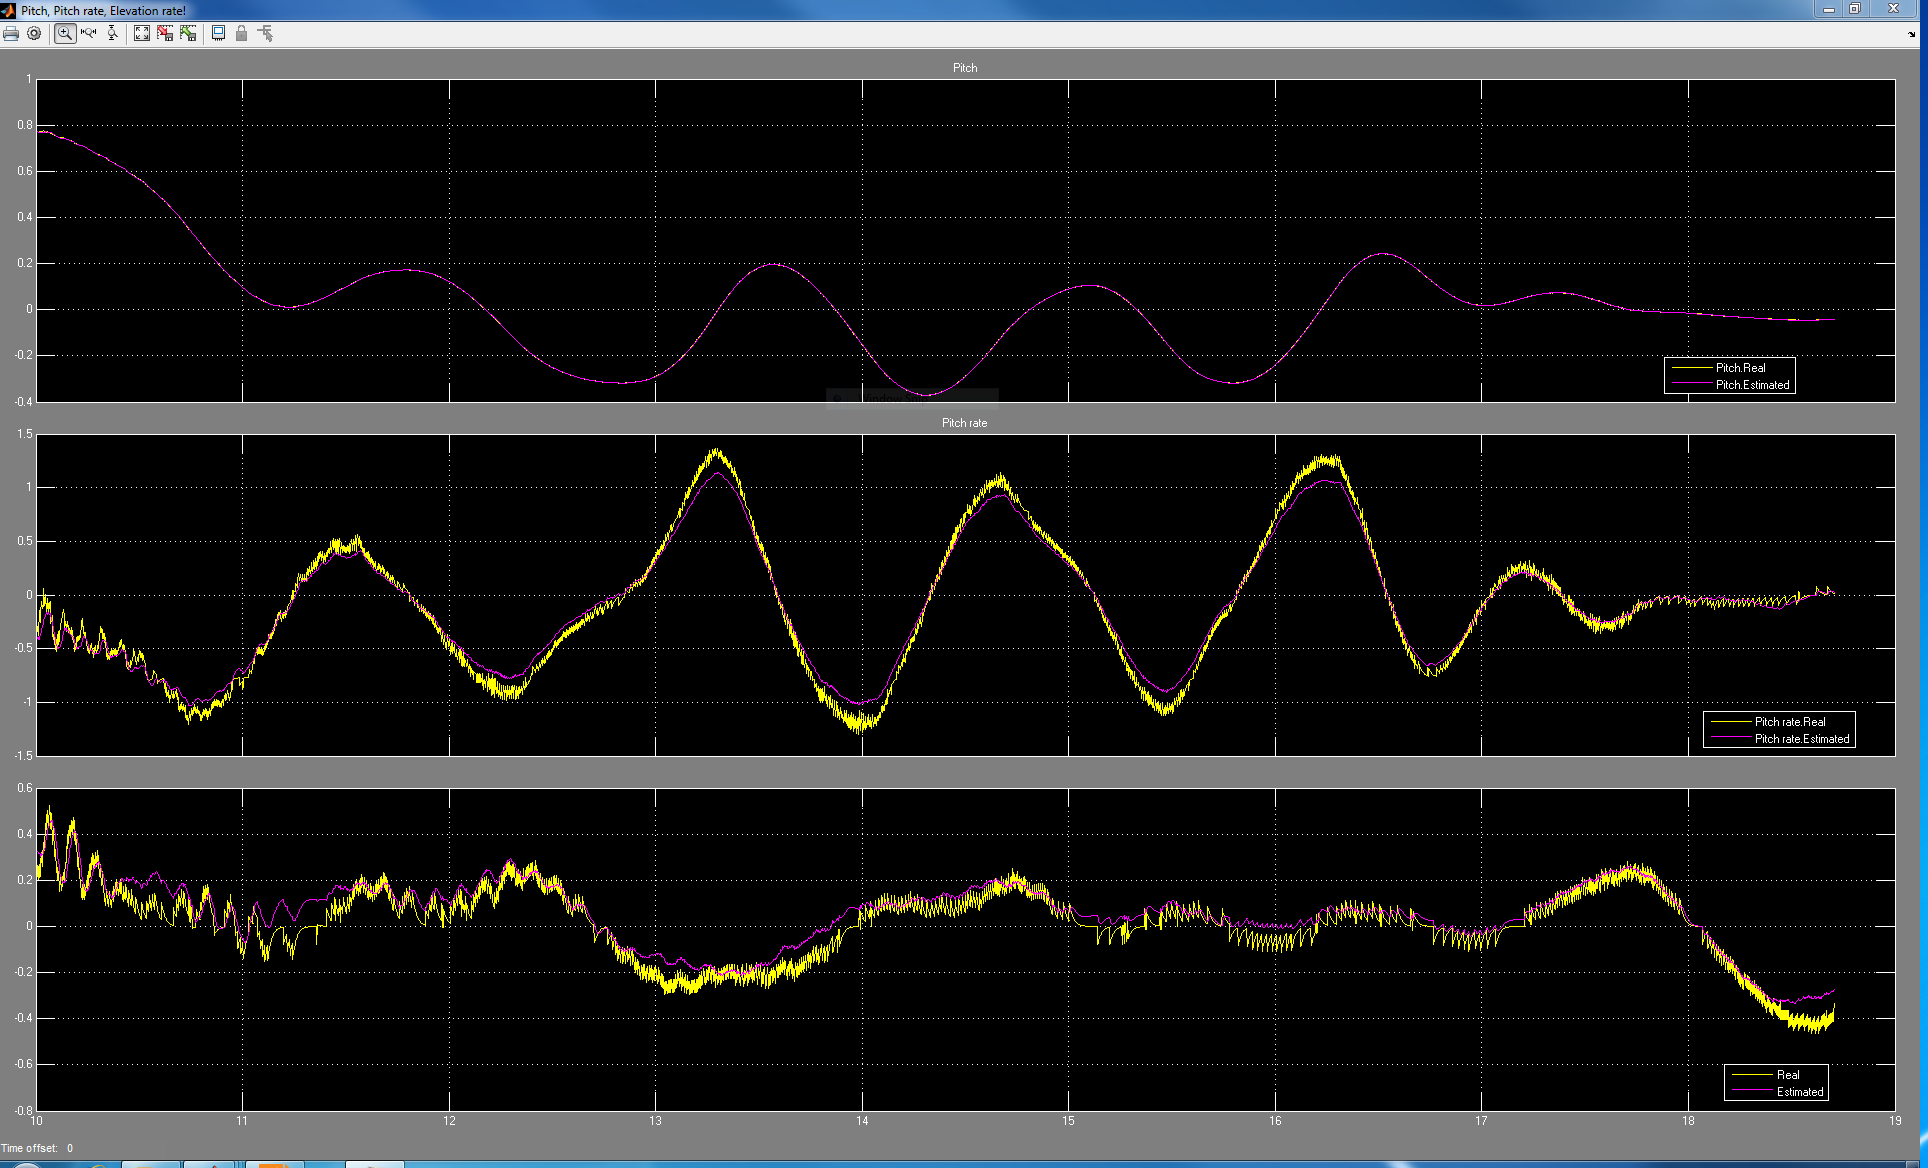
\includegraphics[width=1\textwidth]{figures/superplots_P4p2_del1_best_husk_ratenavn.PNG}
	\caption{Part IV, problem 2 - P controller. Shows the real (yellow) and estimated (purple) states for pitch, pitch rate and elevation rate respectively. As we can see, the estimated states follows the real states quite well.}
\label{fig:P4p2_states_vs_obs}
\end{figure}
\begin{figure}[htb]
	\centering
		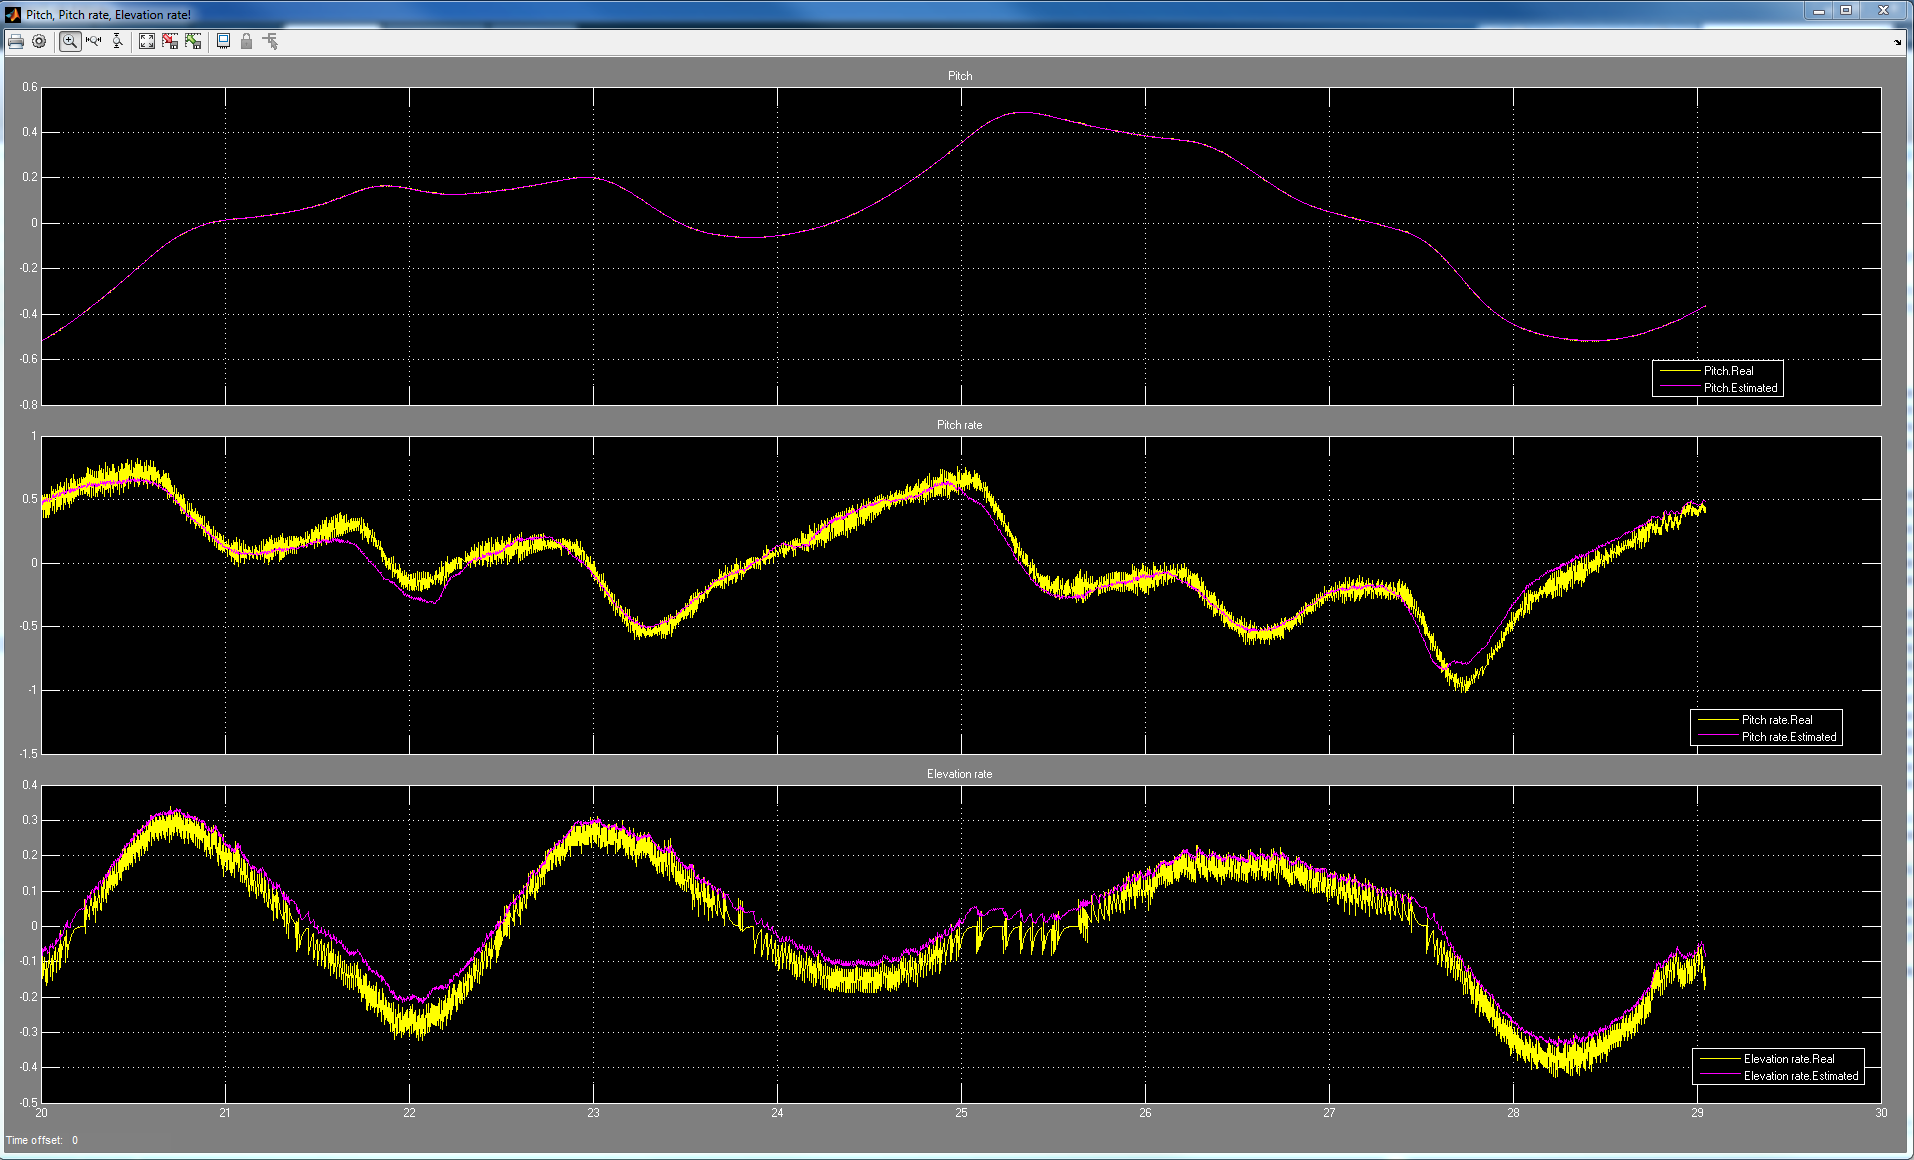
\includegraphics[width=1\textwidth]{figures/superplots_P4p2_del2_integrate_best.PNG}
	\caption{Part IV, problem 2 - PI controller. Shows the real (yellow) and estimated (purple) states for pitch, pitch rate and elevation rate respectively. Again, as we can see, the estimated states follows the real states quite well.}
\label{fig:P4p2_int_states_vs_obs}
\end{figure}
\begin{figure}[htb]
	\centering
		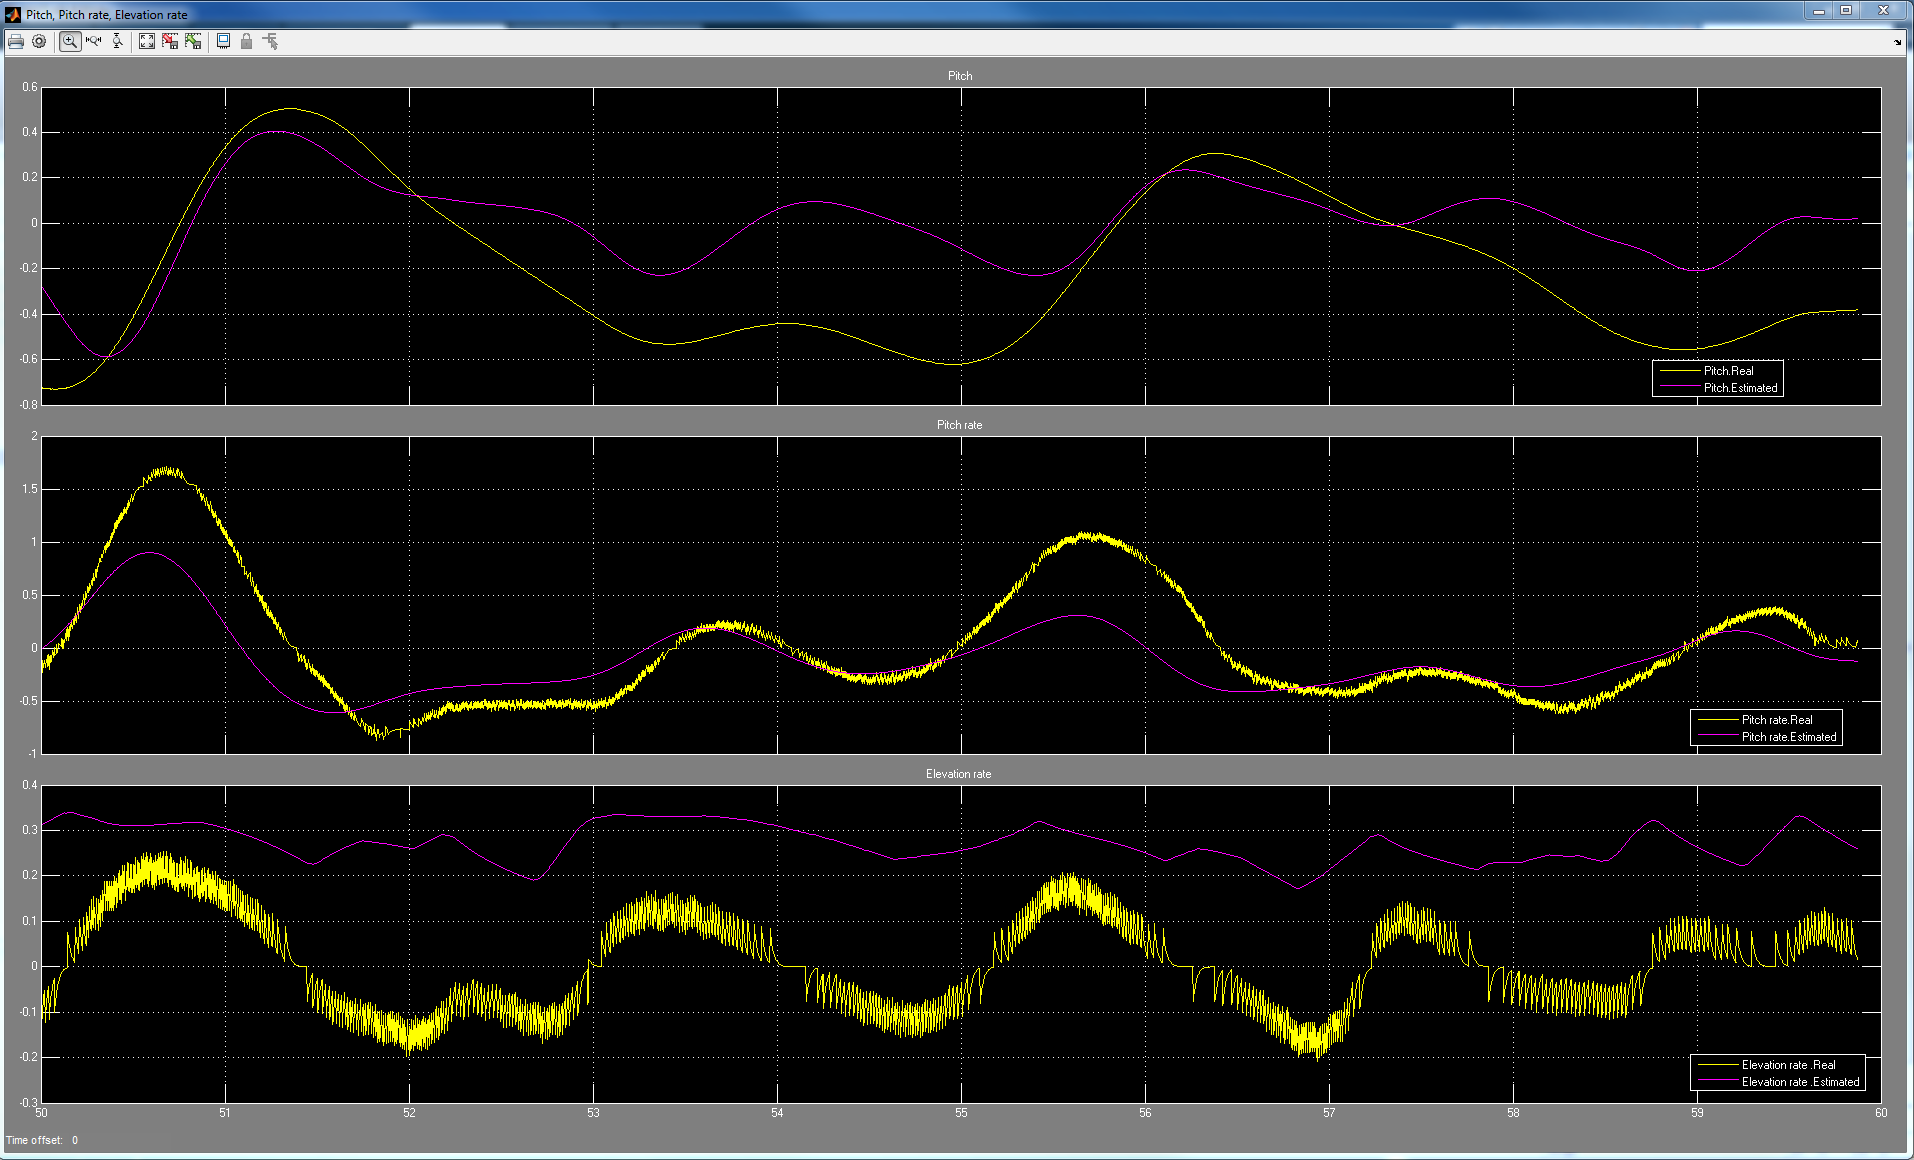
\includegraphics[width=1\textwidth]{figures/superplots_P4p3.PNG}
	\caption{Part IV, problem 3. Shows the real (yellow) and estimated (purple) states for pitch, pitch rate and elevation rate respectively. Clearly, this is not an optimal result as the real and estimated states differ quite a bit.}
\label{fig:P4p3}
\end{figure}

\section{Conclusion}\label{sec:conclusion}
This does not have to be long, but try to write a few reasonable closing remarks.

\addcontentsline{toc}{section}{Appendix} % Remove this if you don't want the appendix included in the table of contents.
\appendix

\section{MATLAB Code}\label{sec:matlab}
This section should contain your MATLAB code. DO NOT attach files posted online (that you didn't write). Note that the method used to input code below does not look as pretty when the lines are too long.

\subsection{plot\_constraint.m}\label{sec:plot_constraint_m}
\lstinputlisting{code/plot_constraint.m}\section{Simulink Diagrams}\label{sec:simulink}
This section should contain your Simulink diagrams. Just like the plots, these should be in vector format, like in \Cref{fig:simulink}. Make them tidy enough to understand.

\subsection{A Simulink Diagram}
\Cref{fig:simulink} shows a Simulink diagram. You can use the \texttt{print\_simulink.m} function, included in the source code repository for this document, to export a Simulink model to EPS\@.
\begin{figure}[htb]
	\centering
		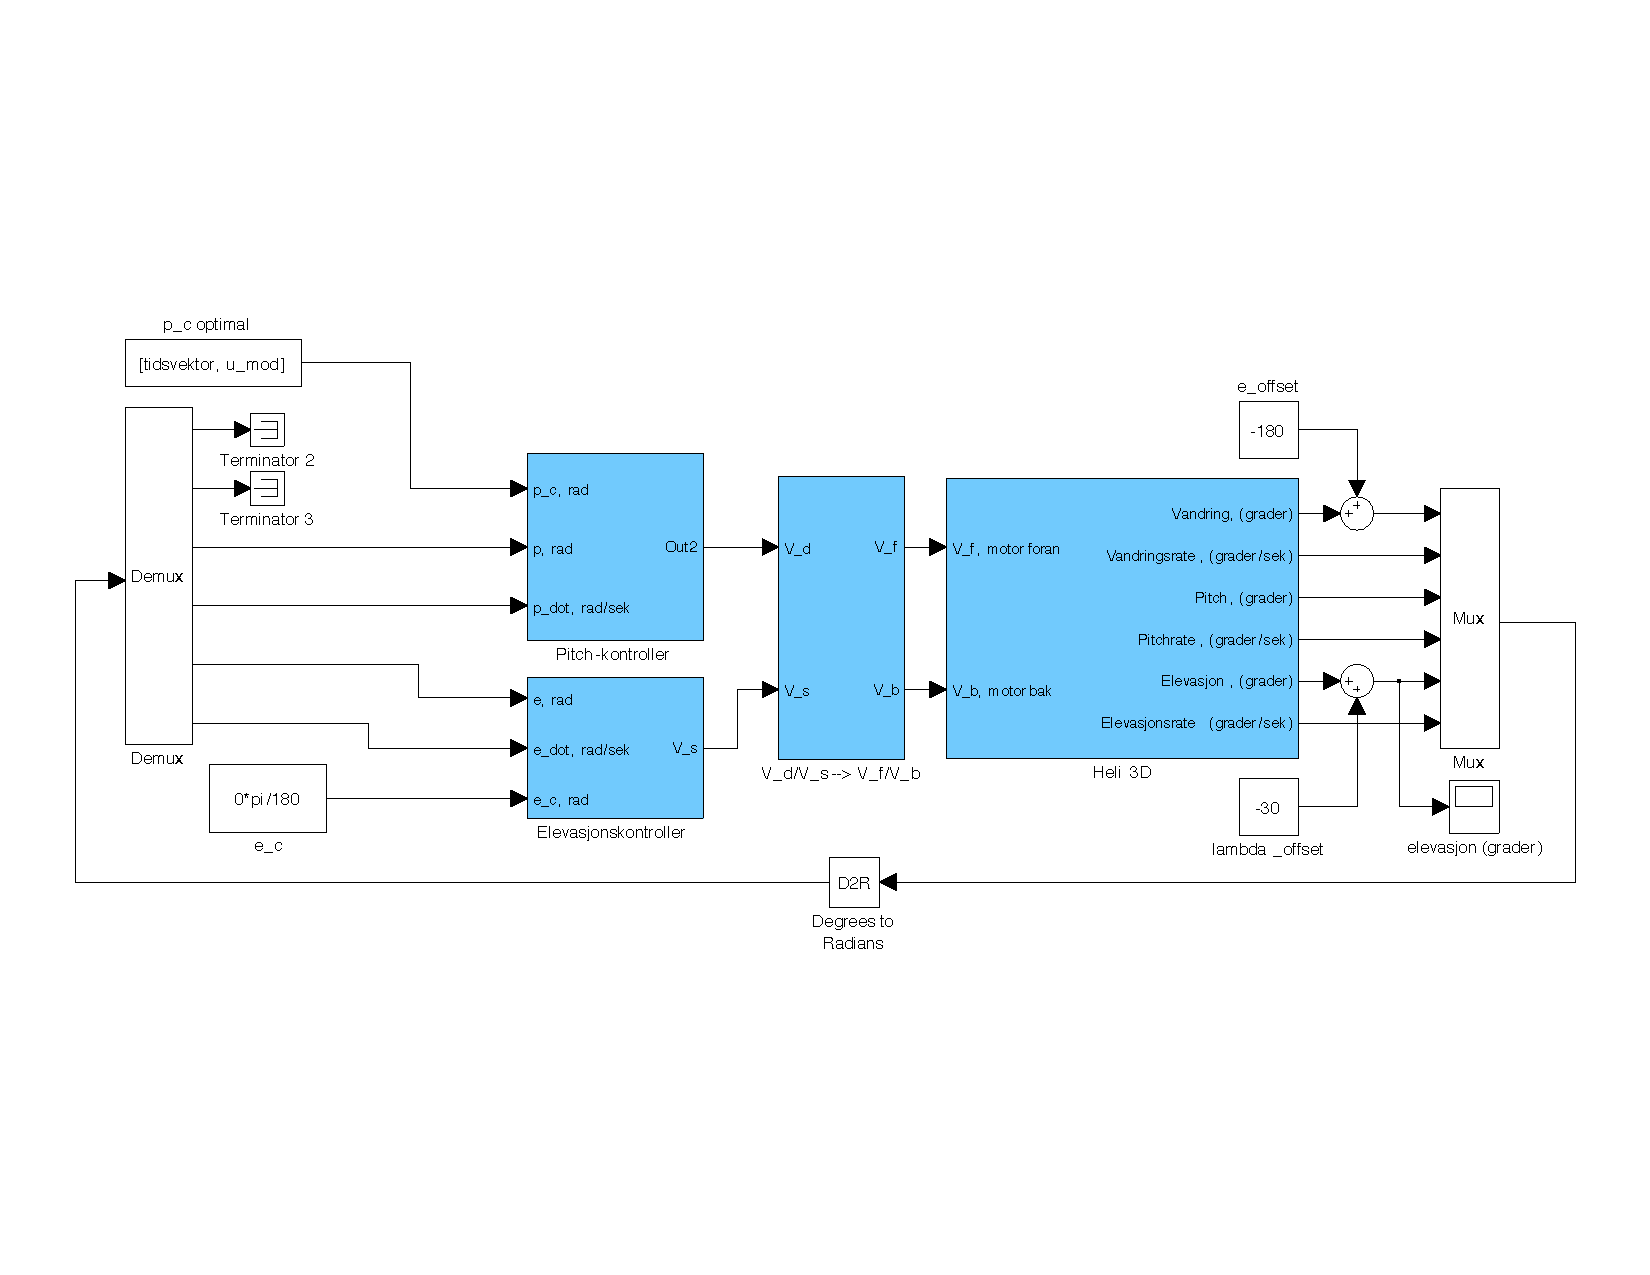
\includegraphics[width = \textwidth]{figures/simulink_fra_mal.pdf}
	\caption{A Simulink diagram.}
\label{fig:simulink}
\end{figure}

% \input simply inserts the contents of the file, while \include forces a \newpage.
% See \input vs. \include: http://tex.stackexchange.com/questions/246/when-should-i-use-input-vs-include

% References
\newpage
\addcontentsline{toc}{section}{References}
\printbibliography{}
\label{sec:bibliography}

\end{document}
